\documentclass[12pt,a4paper,twoside,openright]{article}

\usepackage[a4paper,left=2.8cm,right=2.8cm,top=2.8cm,bottom=2.8cm]{geometry}
%\documentclass[paper=a4, fontsize=11pt]{scrartcl} % A4 paper and 11pt font size

\usepackage[T1]{fontenc} % Use 8-bit encoding that has 256 glyphs
%\usepackage{fourier} % Use the Adobe Utopia font for the document - comment this line to return to the LaTeX default
\usepackage[english]{babel} % English language/hyphenation
\usepackage[utf8]{inputenc}  %allows non-English characters
\usepackage{amsmath,amsfonts,amsthm, amssymb, mathrsfs, yfonts} % Math packages
\usepackage{float}

\usepackage{titlesec}
\usepackage{indentfirst}
\usepackage{caption}
\usepackage{subcaption}
\usepackage[nottoc]{tocbibind}

\usepackage{verbatim}
\usepackage{titlesec}
\usepackage{longtable}
\usepackage{listings}
\usepackage{fancyvrb}
\fvset{frame=single,framesep=1mm,commandchars=\\\{\}}
\usepackage[pdftex]{hyperref,color,graphicx}
%\usepackage[pdftex]{hyperref}
\usepackage{import}
%\usepackage[pdftex,bookmarks,colorlinks]{hyperref}
\usepackage{url}
\usepackage[usenames,dvipsnames]{xcolor}
\usepackage{rotating}
\usepackage{colortbl}
\usepackage{array}
\usepackage[Conny]{fncychap}
\usepackage{listings}
\usepackage{caption}
\renewcommand{\lstlistingname}{Code}
\makeatletter
\renewcommand{\DOCH}{%
    \vskip -4.5\baselineskip
    \mghrulefill{3\RW}\par\nobreak
    %\vskip -0.5\baselineskip
    \mghrulefill{\RW}\par\nobreak
    \CNV\FmN{\@chapapp}\space \CNoV\thechapter
    \par\nobreak
    \vskip -0.5\baselineskip
   }
  \renewcommand{\DOTI}[1]{%
    \mghrulefill{\RW}\par\nobreak
    \CTV\FmTi{#1}\par\nobreak
    \vskip 30\p@
    }
  \renewcommand{\DOTIS}[1]{%
    \mghrulefill{\RW}\par\nobreak
    \CTV\FmTi{#1}\par\nobreak
    \vskip 60\p@
    }
\makeatother

% subfigure and wrapping on figures
\usepackage{subcaption}
\usepackage{wrapfig}

\usepackage[intoc]{nomencl}
\makenomenclature

\hypersetup{
pdftitle={Anonymous Threshold Signatures},
pdfauthor={Hlad Colic, Petar},
%pdfsubject={},
%pdfkeywords={},
colorlinks,
linkcolor=black,
citecolor=black,
urlcolor=blue,
unicode=false
}

\usepackage{fancyhdr} % Custom headers and footers
\pagestyle{fancyplain} % Makes all pages in the document conform to the custom headers and footers
\renewcommand{\sectionmark}[1]{\markright{\thesection\ #1}}
\fancyfoot[LE,RO]{\thepage}
\fancyfoot[C]{}
\fancyhead[RO]{\footnotesize\bfseries}
\fancyhead[LE]{\footnotesize\bfseries}
%\fancyhead[LO,RE]{}

\setcounter{secnumdepth}{4} 
\graphicspath{{../figs/}}

%Include degree symbol in plain text
\usepackage{gensymb}


%Notes on the page (toggle last lines)
\usepackage[colorinlistoftodos]{todonotes}
\setlength{\marginparwidth}{2cm}
\newcommand{\mytodo}[1]{\todo[size=\footnotesize]{#1}}

%\usepackage{biblatex}
\usepackage{enumitem}

\usepackage{flafter}
\usepackage{multirow}
\newcolumntype{M}[1]{>{\arraybackslash}p{#1}}
\newcolumntype{N}{@{}m{0pt}@{}}
\usepackage{pbox}
\usepackage[gen]{eurosym}
%\newcommand{\euro}{euroWARNING}

\lstdefinestyle{tt}{
breakatwhitespace=true,
breaklines     = true,
  frame=top,frame=bottom,
  basicstyle=\small\normalfont\sffamily,    % the size of the fonts that are used for the code
   stepnumber=1,
   numbersep=10pt,                     % how far the line-numbers are from the code
   numbers=left,
   numberstyle=\tiny\color{gray},
  tabsize=2,                              % tab size in blank spaces                     %
  breaklines=true,                        % sets automatic line breaking
  captionpos=t,                           % sets the caption-position to top
    showspaces=false,           % Leerzeichen anzeigen ?
  showtabs=false,             % Tabs anzeigen ?
  xleftmargin=17pt,
  framexleftmargin=17pt,
  framexrightmargin=17pt,
  framexbottommargin=5pt,
  framextopmargin=5pt,
  showstringspaces=false
 }
\DeclareCaptionFormat{listing}{#1#2#3}
\captionsetup[lstlisting]{format=listing,singlelinecheck=false, margin=0pt, font={sf}}

\usepackage{adjustbox}

\usepackage{pdfpages}
\usepackage{afterpage}

% I only need the arrows for this one.
\usepackage{tikz}
\usetikzlibrary{arrows}

% Package to strikeout text
\usepackage[normalem]{ulem}

%shortcuts for typing variance and expectation

\newcommand{\Var}{\mathrm{Var}}
\newcommand{\FF}{{\mathbb F}}
\newcommand{\RR}{{\mathbb R}}
\newcommand{\ZZ}{{\mathbb Z}}
\newcommand{\PP}{{\mathcal P}}
\newcommand{\A}{{\mathcal A}}
\newcommand{\E}{\mathcal{E}}
\newcommand{\D}{\mathcal{D}}
\newcommand{\K}{\mathcal{K}}
\newcommand{\G}{\mathcal{G}}
\newcommand{\M}{\mathcal{M}}
\newcommand{\C}{\mathcal{C}}
\newcommand{\acc}{\Gamma}
\newcommand{\con}{\! \parallel \!}
\newcommand{\cl}{\text{cl}}
\newcommand{\KK}{\mathcal{K}}
\newcommand{\kk}{\mathbf{k}}
\renewcommand{\SS}{\mathcal{S}}
\newcommand{\F}{{\mathscr F}}
\newcommand{\s}{{\mathfrak s}}
\renewcommand{\i}{{\mathfrak i}}
\renewcommand{\v}{{\mathfrak v}}

\newcommand{\card}[1]{\left\vert {#1} \right\vert}

\theoremstyle{plain}
\newtheorem{thm}{Theorem}[section]
\newtheorem{cor}[thm]{Corollary}
\newtheorem{prop}[thm]{Proposition}

\theoremstyle{definition}
\newtheorem{prob}[thm]{Problem}
\newtheorem{defn}[thm]{Definition} 
\newtheorem{exmp}[thm]{Example}
\newtheorem{remk}[thm]{Remark}
\newtheorem*{keygen}{Key generation}
\newtheorem*{sign}{Signing}
\newtheorem*{ver}{Verification}
%\usepackage[backend=bibtex, style=alphabetic, maxnames=4, minnames=3, maxbibnames=99]{biblatex}

\usepackage{pdfpages}
\usepackage{appendix}
\usepackage{caption}
\usepackage{subcaption}
%%%%%%%%%%%%%%%%%%%%%%%%%%%%%%%%%%%%%%%%
\DeclareRobustCommand{\hesham}[1]{ {\begingroup\sethlcolor{yellow}\hl{(hesham: #1)}\endgroup} }
\DeclareRobustCommand{\petar}[1]{ {\begingroup\sethlcolor{green}\hl{(petar: #1)}\endgroup} }

\begin{document}

\title{CSAS Project Report \\ Attitude Estimation with Extended Kalman Filter}
% author names and affiliations
\author{Petar Hlad \\
\texttt{petar.hlad@estudiantat.upc.edu}}

\maketitle

    \section{Introduction}
\begin{frame}{Attitude Estimation}

Attitude estimation is the process of estimating the orientation of an aerospace vehicle with respect to an intertial frame of reference. \\~\\

Usually, in navigation, attitude is estimated with 3 angles:
\begin{itemize}
\item \textbf{Yaw}: angle respect to true north. Heading.
\item \textbf{Pitch}: angle of the nose respect to the horizon. Angle of attack.
\item \textbf{Roll}: angle of the wings respect to the horizon. Bank.
\end{itemize}

\begin{center}
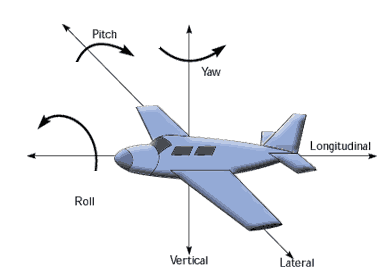
\includegraphics[width=0.5\textwidth]{figures/attitude.png}
\end{center}
\end{frame}


\begin{frame}{Sensors}
To perform attitude estimation, sensors are needed:
\begin{itemize}
\item Accelerometer: gives direction of gravity.
\item Gyroscope: gives rate of turn.
\item Magnetometer: gives direction of magnetic north.
\end{itemize}
\end{frame}
    
    \section{Hardware Setup}
\begin{frame}{Setup}
\begin{itemize}
\item Raspberry Pi 3
\item MPU6050 Accel + Gyro
\item \sout{LSM3030DLHC Accel + Magneto}
\item Communicate through I2C using mpu6050 python library
\end{itemize}

\begin{center}
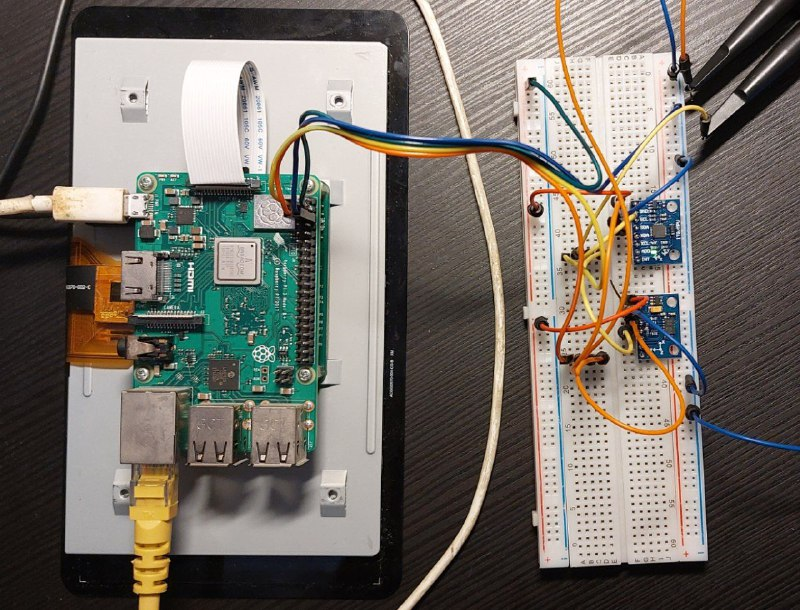
\includegraphics[width=0.4\textwidth]{figures/setup.jpeg}
\end{center}
\end{frame}

\begin{frame}{Issues}
\begin{itemize}
\item Magnetometer not working.
\item Only pitch and roll.
\end{itemize}
\end{frame}
    
    \section{System Formulation}
To apply Kalman Filter to the measured sensor data, we first need to find the functions and matrices that model our dynamic system. These are the state vector $x$, measurement vector $z$, update function $f$, measurement function $h$ and differential matrices $F$ and $H$.

\begin{equation}
    \label{eq:non_linear_update}
    x_{k} = f( x_{k-1}, u_k) + v_k
\end{equation}

\begin{equation}
    \label{eq:non_linear_meas}
    y_k = h (x_k) + w_k
\end{equation}

\begin{equation}
    F = \left. \frac{\partial f(x)}{\partial x} \right\vert_{x = x_{k-1}}; \quad
    H = \left. \frac{\partial h(x)}{\partial x} \right\vert_{x = x_{k}}
\end{equation}

\subsection{Euler Angles}
An important concept to find the description of the system are the Euler angles. The Euler angles are used to describe the orientation of a rigid body with respect to a fixed coordinate system.
Since we are not using magnetometer, we will just take into account pitch and roll ($\theta$ and $\phi$ respectivelly).

\begin{figure}[h]
\centering
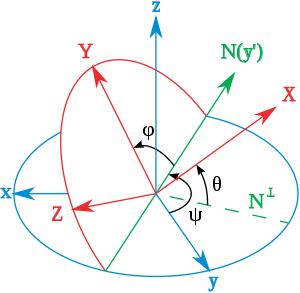
\includegraphics[width=0.4\textwidth]{figures/brian.png}
\caption{Euler angles}
\label{fig:euler}
\end{figure}

\subsection{Formulation}
Even though we are not measuring yaw ($\psi$), we still take it to acount in the system states since it does have an impact in giroscopic measures. The system state is defined in equation \ref{eq:system}

\begin{equation}
    \label{eq:system}
    x_k = 
        \begin{pmatrix}
            \varphi_k \\
            \theta_k \\
            \psi_k
        \end{pmatrix}
\end{equation}

The accelerometer measurements will be transformed to attitude measurements through a simple transformation defined in equation \ref{eq:meas}. It is simply the angles in two directions of the gravity vector with the $xy$ plane of the sensor.

\begin{equation}
    \label{eq:meas}
    z =
    \begin{pmatrix}
        \theta\\
        \varphi
    \end{pmatrix}
    = 
    \begin{pmatrix}
        asin \left( \frac{a_x}{g} \right) \\
        asin \left( -\frac{a_y}{g \cos \theta} \right)
    \end{pmatrix}
\end{equation}

Consequently, the expression of $H$ following equation \ref{eq:non_linear_meas} is very simple, and is defined in equation \ref{eq:H}

\begin{equation}
\label{eq:H}
H =
\begin{pmatrix}
1 & 0 & 0 \\
0 & 1 & 0
\end{pmatrix}
\end{equation}

To complete the formulation, we need to relate the angular rates measured by the gyroscope with the system state.
We need a transformation between the angular rates from gyroscope and the angular velocities of the fixed frame.

In \cite{ekf} it is described transformation defined in equation \ref{eq:euler_transf}. To obtain the transformation from gyroscope angular rates to euler angle velocities, we just need to invert the matrix from equation \ref{eq:euler_transf} and obtain the one in equation \ref{eq:T}.

To clarify the notation used in equations \ref{eq:euler_transf} and \ref{eq:T}:
\begin{itemize}
\item $\dot{\varphi}$, $\dot{\theta}$ and $\dot{\psi}$ are the angular velocities of the fixed frame
\item $p$, $q$ and $r$ are the angular rates from the gyroscopes.
\end{itemize}

\begin{equation}
    \label{eq:euler_transf}
    \begin{pmatrix}
        p \\
        q \\
        r
    \end{pmatrix}
    = \begin{pmatrix}
        1 & 0 & -\sin \theta \\
        0 & \cos \varphi & \sin \varphi \cos \theta \\
        -\sin \varphi & 0 & \cos \varphi \cos \theta
    \end{pmatrix}
    \begin{pmatrix}
        \dot{\varphi} \\
        \dot{\theta} \\
        \dot{\psi}
    \end{pmatrix}
\end{equation} 

\begin{equation}
    \label{eq:T}
    \dot{x} =
    \begin{pmatrix}
        \dot{\varphi} \\
        \dot{\theta} \\
        \dot{\psi}
    \end{pmatrix}
    = \begin{pmatrix}
        1 & \sin \varphi \tan \theta & \cos \varphi \tan \theta \\
        0 & \cos \varphi & - \sin \varphi \\
        0 & \frac{\sin \varphi}{\cos \theta}  & \frac{\cos \varphi}{\cos \theta}
    \end{pmatrix}
    \begin{pmatrix}
        p \\
        q \\
        r
    \end{pmatrix}
\end{equation} 

At this point, the update function can be defined as in equation \ref{eq:update}, which is just the previous state plus the state variation during a time step.

\begin{equation}
\label{eq:update}
f(x,p,q,r,dt) = x + T
\begin{pmatrix}
p \\ q \\ r
\end{pmatrix}
dt = x + \dot{x} dt
\end{equation}

Finally, the differencial matrix of $f$ looks very complicated (equation \ref{eq:F}) , but it is just computed taking the derivatives of $f$ with respect to the euler angles (not the angle rates from the sensors).

\begin{equation}
    \label{eq:F}
   F = I + dt
   \begin{pmatrix}
       q \cos\varphi \tan\theta - r \sin\varphi \tan \theta &
       q \sin \varphi \sec^2 \theta + r \cos \varphi \sec^2 \theta &
       0 \\
       -q \sin \varphi - r \cos \varphi
       & 0 & 0 \\
       q \cos \varphi \sec \theta - r \sin \varphi \sec \theta &
       q \sin \varphi \sec \theta \tan \theta + r \cos\varphi \sec \theta \tan  \theta &
       0
   \end{pmatrix}
\end{equation}


\subsection{Extended Kalman Filter}
Just as a reminder, the steps to perform the Extended Kalman Filter are depicted in equation \ref{eq:ekf}, for our defined system, and covariance matrices Q and R.
\begin{equation}
\label{eq:ekf}
\begin{array}{c}
    \hat{x}_k = f(x_{k-1},p,q,r,dt) \\
    \hat{P_k} = F_k P F_k' + Q \\
    K_k = \hat{P_k} H \left(H \hat{P_k} H' + R\right)^{-1} \\
    x_k = \hat{x}_k + K_k \left(z_k - H \hat{x}_k \right) \\
    P_k = \hat{P}_k - K H \hat{P}_k 
\end{array}
\end{equation}

The code used to compute the output of the Extended Kalman Filter has been implemented following the explanations from \cite{kim2011kalman} and can be found in \cite{repo}.
    
    \section{Measurements}

First thing to do with the measurements is to subtract the bias from the sensor data. For this, the sensor has been put on a flat surface and recorded 500 samples along 10 seconds. The values have been averaged to obtain the bias (see table \ref{tab:bias}) and later subtracted to any following Kalman Filtering.

\begin{table}[h]
    \centering
    \begin{tabular}{|c|c|c|c|}
    \hline
    Sensor bias & x & y & z\\ \hline
    Accelerometer $(m/s^2)$ & 0.817012 & -0.045973 & 10.379578 \\ \hline
    Gyroscope ($\degree/s$) & -0.0170254 &  0.0262836 & -0.0076507 \\
    \hline
\end{tabular}
    \caption{Sensor measurement bias measured on flat surface.}
    \label{tab:bias}
\end{table}

To test the setup, the sensor has been handheld and rotated first 45 degrees roll in each direction, and then 45 degrees pitch in each direction. In figure \ref{fig:sensor_data} we can see the raw data from the accelerometer and the gyroscope.

\begin{figure}[h]
\centering
\begin{subfigure}[b]{0.45\textwidth}
    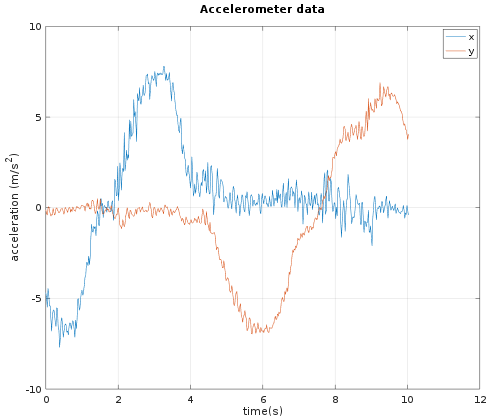
\includegraphics[width=\textwidth]{figures/acc_data.png}
    \caption{Accelerometer measurements}
    \label{fig:acc_data}
\end{subfigure}
\begin{subfigure}[b]{0.45\textwidth}
    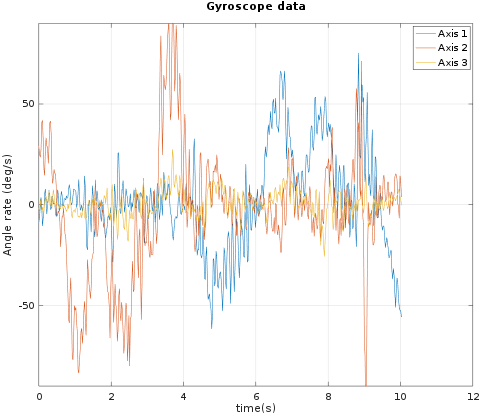
\includegraphics[width=\textwidth]{figures/gyro_data.png}
    \caption{Gyroscope measurements}
    \label{fig:gyro_data}
\end{subfigure}
\caption{Raw Sensor data}
\label{fig:sensor_data}
\end{figure}

Then we apply Extended Kalman Filter to the data and obtain the results in figure \ref{fig:kalman_results}. Figure \ref{fig:acc_attitude} is the estimated attitude computed directly from the accelerometer data using equation \ref{eq:meas}. Figure \ref{fig:kalman_results} is the estimated attitude obtained from the output of the Extended Kalman Filter. We can see it is much smoother than the attitude from the accelerometer data.

\begin{figure}[h]
\centering
\begin{subfigure}[b]{0.45\textwidth}
    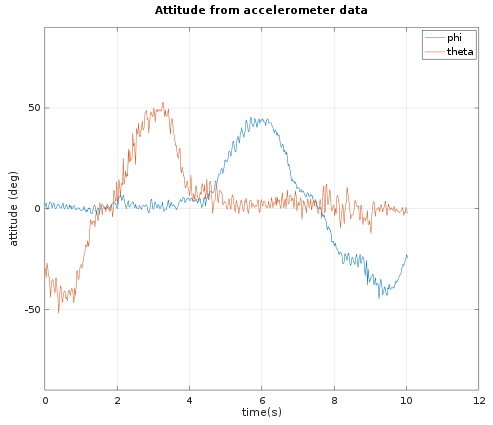
\includegraphics[width=\textwidth]{figures/acc_attitude.png}
    \caption{Attitude from accelerometer.}
    \label{fig:acc_attitude}
\end{subfigure}
\begin{subfigure}[b]{0.45\textwidth}
    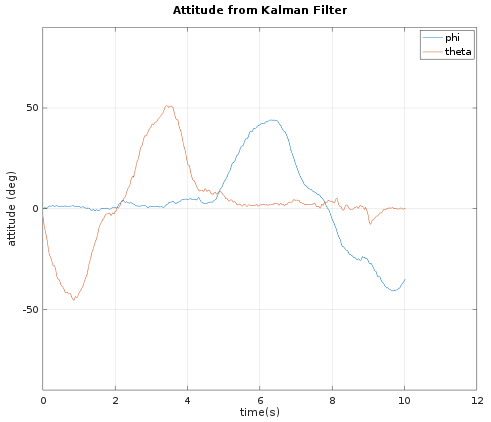
\includegraphics[width=\textwidth]{figures/attitude_kalman.png}
    \caption{Attitude from Kalman Filter}
    \label{fig:attitude_kalman}
\end{subfigure}
\caption{Attitude estimation}
\label{fig:kalman_results}
\end{figure}

    
    \section{Conclusions}
\begin{frame}{Conclusions}
\begin{itemize}
\item Kalman Filter is avery good and powerful tool to work with dynamical systems
\item There is a better version for attitude estimation using quaternions on a linear Kalman Filter, but the formulations is more complicated.
\item To evaluate performance of setup, would need other tools to measure actual attitude.
\end{itemize}
\end{frame}

\bibliographystyle{unsrt}
\bibliography{refs}


\end{document}


